%Chapter 2 - Literature Review


\chapter{Literature Review} % Main chapter title
\label{Chapter2} % For referencing the chapter elsewhere, use \ref{Chapter1} 

%----------------------------------------------------------------------------------------
%----------------------------------------------------------------------------------------
\section{Early home computer era}
 
Mid-1970s to late-1980s was an interesting period in the history of computers. It marked the first time computers were designed and marketed for personal use in the home: the early home computer era. Home computer is an ambigous term not defineied by any standard, here it is taken to be synonomus with a microcomputer or a personal computer (PC) from the era.  A PC is classified by Gupta, A. and Toong, H.  as computer that furfills all of the following characteristics \cite{Gupta84}: \\

\begin{enumerate}
\item The computer cost less than US\$5000 at the time of sale.\\
\item The computing power is provided by a microprocessor from the era. \\
\item The computer is sold through mass-marketing channels. \\
\item The computer can run a wide range of programs for varied fields such as industry, business, education and at home; it is not designed for a single purpose or a single type of user.
\item The computer can handle at least one high-level language , such as BASIC, Fortran, or COBOL.
\end{enumerate}

Since the discovery of semiconductors in the 1940s, there have been continuous efforts and advances in making electronic devices smaller, more powerful and cheaper. 1958 saw the first working Integrated Circuit (IC), continuing this trend \cite{Kilby01}. By 1965 Moore was talking about this observation, which came to be popularly known as "Moore's Law" \cite{moore65}. In 1971, Intel developed the first microprocessor; the 4-bit 4004 on a single IC \cite{intel4004}. A microprocessor is an entire CPU within an IC or a few ICs. The following year Intel released the more powerful 8-bit 8008 microprocessor. Then in 1974 the 8080 was released \cite{intelchips}. \\

\begin{figure} \begin{center}
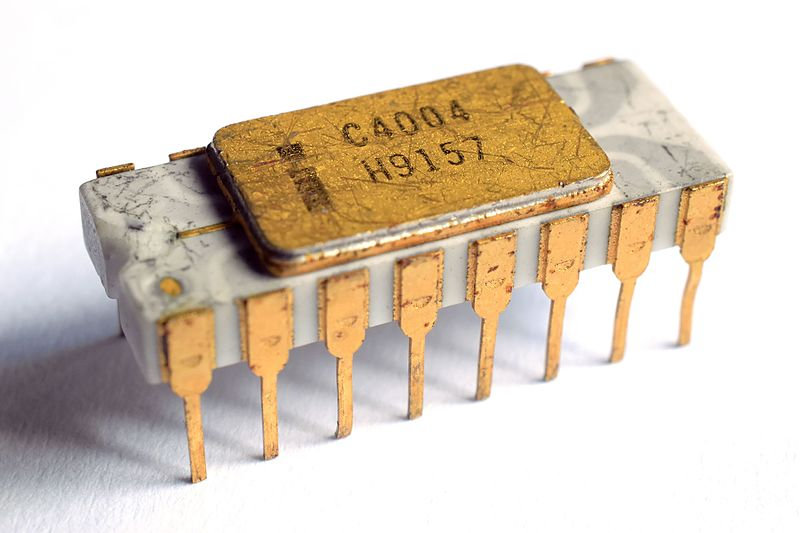
\includegraphics[width=.3\linewidth]{pics/intel_4004} 
\end{center} 
\caption{Intel 4004 microprocessor, an entire CPU on a single chip; the first microprocessor. Released in 1971.\\ \textit{\small{Picture courtesy of Thomas Nguyen}}}
\end{figure} 

%\begin{figure} \begin{center}
%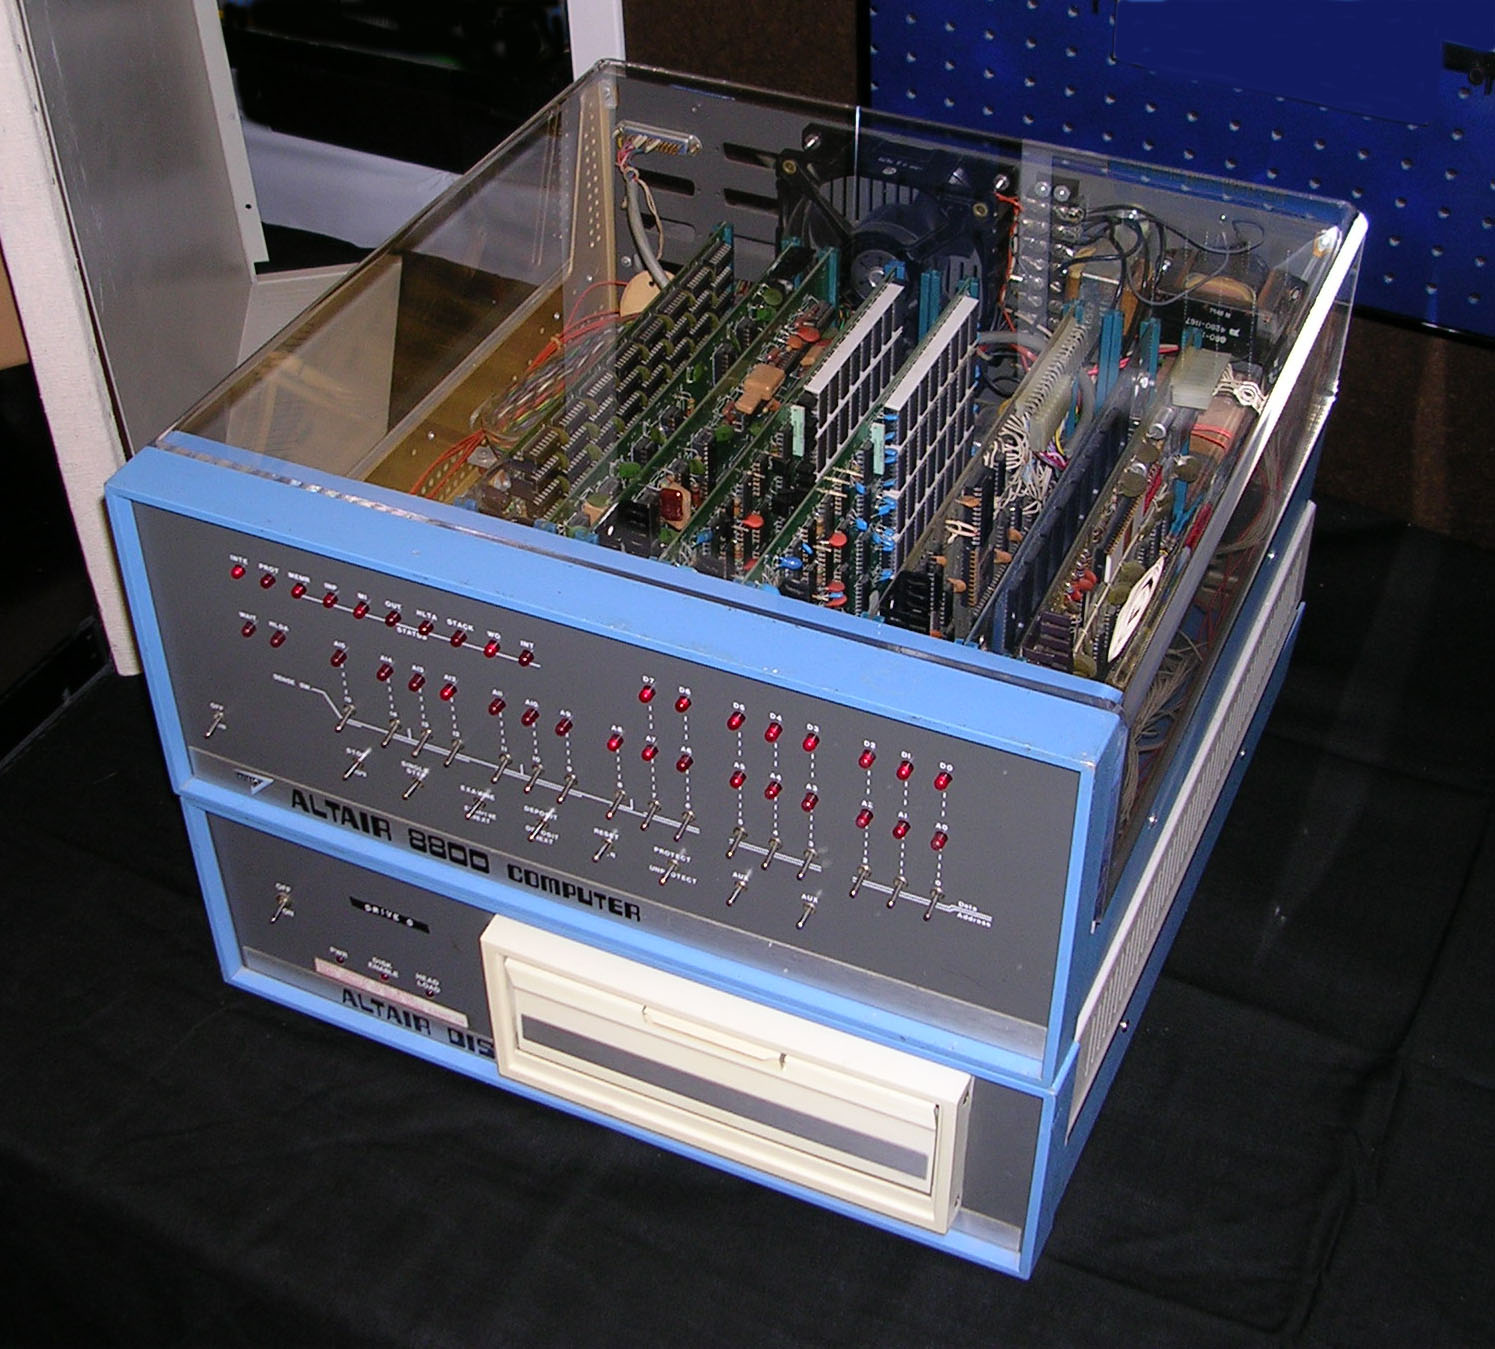
\includegraphics[width=.3\linewidth]{pics/altair_8800_computer}\quad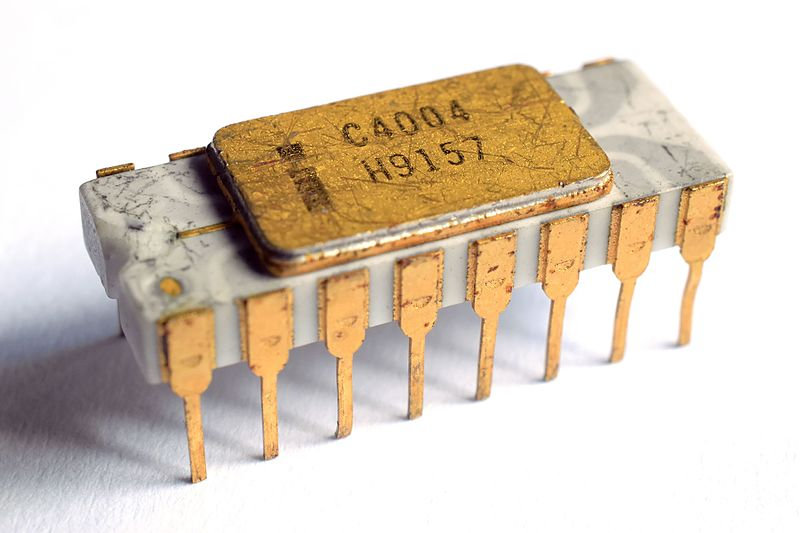
\includegraphics[width=.%3\linewidth]{pics/intel_4004}
%\caption{Left: MITS Altair 8800 home computer. Right: Intel 8080 microprocessor}
%\end{center} \end{figure} 

It seems a tipping point had now been reached, the manufacturing cost of computers was low enough, their size was small enough and their performance was high enough that some manufacturers thought to start selling them to personal users. In 1974 MITS released what can be considered the first market successful home computer \cite{Dorf95}, the Altair 8800 which used an 8080 microprocessor. \\

\begin{figure} \begin{center}
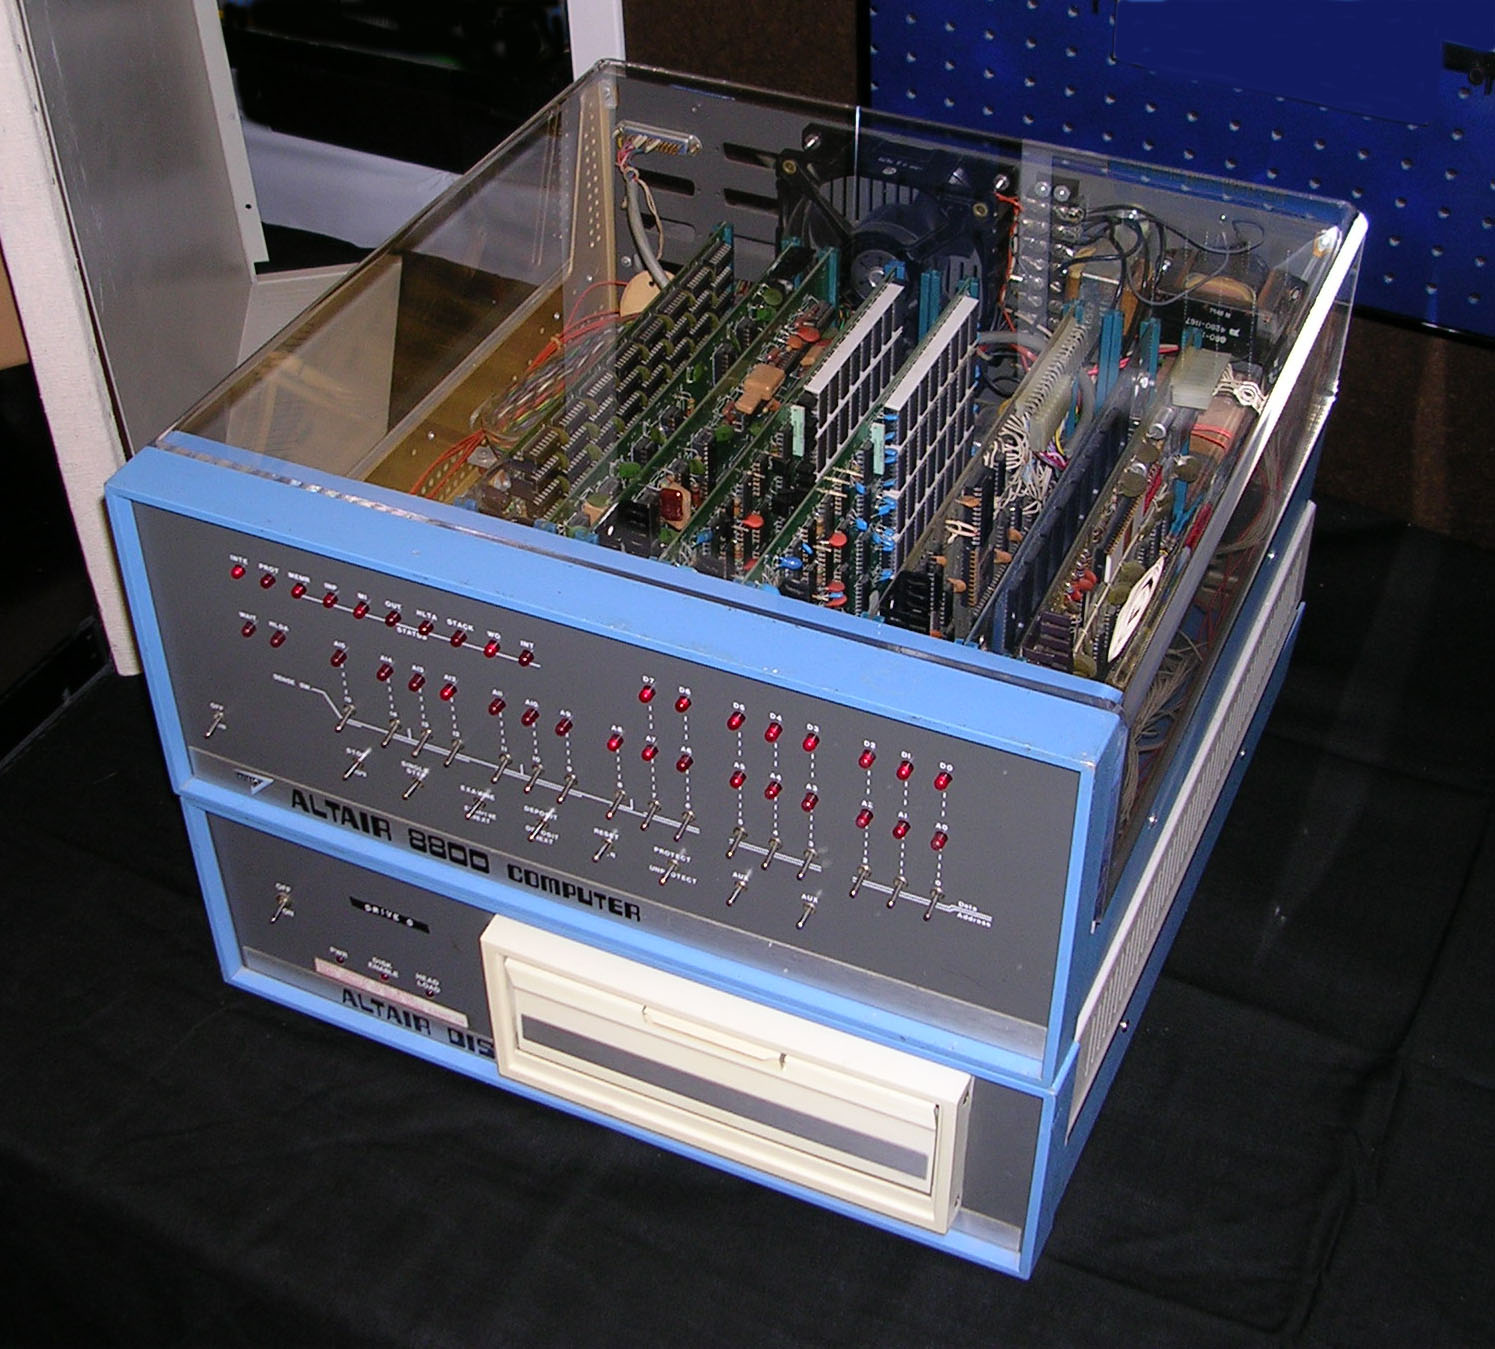
\includegraphics[width=.3\linewidth]{pics/altair_8800_computer} 
\end{center} 
\caption{MITS Altair 8800 home computer, the first market succesful home computer. It used an 8-bit 8080 microprocessor and was released in 1974.\\ \textit{\small{Picture courtesy of  Michael Holley}}}
\end{figure}

Over the next 15 or so years, a flurry on new companies sprung up, offering a multitude of personal computers \cite{Micro}. New microprocessors where developed, further increase performance and reducing cost. The most notably of these is the 8-bit 6502 by MOS Technology, which when released in 1975, was the least expensive microprocessor on the market \cite{EET75}. A sense of excitment and seemingly an expectation that computers where going to revolutionise society was abound at this time \cite{Cass14}. Many people where having their first interations with computers as the home computer became more wide spread. These computers had a relatively simple interface, when compared to modern computers. This meant there was far less abstraction between the user and the inner workings of the computer, this may have allowed their users to more readily understand the underlying mechanisms. It also meant that users had to learn at least some rudimentry programming skills to use them. Users could get programs by typing them into their own computers out of magazines or from computer shows on TV. Most of the home computers in this period ran some form of BASIC. There where some people that questionioned the usefulness of the early home computers, and with some merit, as there was a lack of software during the begining of the era \cite{Swalwell12}. Others still had frankly unrealistic expectations of what computers would do for them. These home computers where mainly used in a four areas: business, science and engineering, education and in the home. Business, science and engineering uses included manipulating spreadsheets, word processing, basic graphics, databases and communication to connect to host computer or LANs. In home, the most widely reaching use of these home computers was to play games \cite{Gupta84}. These 8-bit home computers were where many first met and became interested in the potential of computers and computer programming and they helped kick off a revolution.


%----------------------------------------------------------------------------------------
%----------------------------------------------------------------------------------------
\section{Commodore 64, 128, 65}
\subsection{Commodore 64}
The Commodore 64 was one of the most successful home computers, selling over 17 million units according to Commodore Intentional \cite{pagetable}, the now defunct manufacturers of the Commodore 64. Earning it  a Guinness world record (formally Guinness Book of Records) 'Most computer sales' \cite{guinness}
It was released in January 1982 \cite{infoworld82}. The computational power came from a 8-bit MOS Technology 6510 microprocessor, a modified version of the 6502 mentioned earlier. It had 64 kilobytes of RAM which was the inspiration of its name. The Commodore 64 was a dominate market presence in its time, it sold for US\$595 at launch. In a category of influential computers (home computers), the Commodore 64 may well have been the most influential of all. It ran a version of BASIC and there was a huge software library created during its lifetime.

\subsection{Commodore 128}
The Commodore 128 was Commodore Internationals innovation of the very successful Commodore 64. Released in January, 1985. It was meant to build on the success of the 64 by bringing some innovations while still being near 100\% compatible with Commodore 64 software. It was powered by a more powerful 8-bit 8502 microprocessor and had 128 kilobytes of RAM. An innovation was the inclusion of a second microprocessor, an 8-bit Zilog Z80. This second CPU allowed the 128 to run CP/M (an operating system of the time) as well as the Commodore BASIC environment similar to the 64. Running CP/M as well allowed the 128 to access the CP/M software library, which was quite extensive, as well as the Commodore 64 software library, giving the 128 one of the broadest ranges of software compared to its competitors of the day.

\subsection{Commodore 65}
The Commodore 65 was in development in 1990-1991, when Commodore Business Machines (subsidiary of Commodore Intentional) went bankrupt in 1994 a number of prototypes where sold on the market. It was planned to be an upgrade of the 64. Compute! Gazette reported in an article in 1989 that the C65 had a 16-bit 65816 microprocessor; a 16-bit version of the 6502 \cite{gazette89}. Years later when the prototypes where sold, other sources report a modified 65CE02 microprocessor was used (gardner-stephen, secret weapon page). The 65CE02 was an 8-bit CPU with a limited ability to address 16-bit words. It had 128 kilobytes of RAM, expandable to 1 megabyte. It had a 'stunning' 640x400 pixel maximum resolution \cite{gazette89}. It had a 64 compatibility mode, meant to allow near 100\% compatibility with the 64 but there have been some doubts cast on this (secret weapon, gardner-s). It had a VIC-III graphics chip.

%----------------------------------------------------------------------------------------
%----------------------------------------------------------------------------------------
\section{History of the MEGA65 project}
Started sometime before January 2014 by Dr. Paul Gardner-Stephen \cite{blogjan14}, the MEGA65 project is attempting to innovate the Commodore 65 with near 100\% compatibility with C64 software. Dr. Gardner-Stephen  owned a Commodore 65 prototype between 1994-2010, he also owned a Commodore 128 through the same time and when compared, preferred the C65. Dr. Garnder-Stephen also loved to tinker with these computers during the 1990 and 2000s, devising ways of accelerating the C64 CPU(clock speed?) as an example. After deciding to sell the C65 prototype to a collector for various reasons, not least of which was their ability to maintain it better, Dr. Gardner-Stephen always had the idea of recreating the C65 and implement some of the tricks and ideas he had worked out or heard of over the years. Then, during Dr. Gardner-Stephen's PhD studies, he leart to program in VHDL and it seemed possible to realise this dream using the technogy of FPGAs. This dream was delayed still by technological issues with the FPGA boards of the time not quite being fast enough for Dr. Gardner-Stephen's vision. But by 2013, a sufficient board had been released to the market. \\\\

Dr. Gardner-Stephen chose a Nexys4 development board, used by a lot of teaching institutions and designed with students in mind. This FPGA has many built in peripherals which can be used by the computer as well as its cost to performace ratio makes it ideal. The added benefit of using off-the-shelf FPGA board is that availability should be much greater compared to a PCB created just for MEGA65, which would be limited to small production runs carried out by the MEGA65 team or at their request \cite{blog30jan14}. \\\\

The MEGA65 project is completely open-source with the hardware VHDL/verilog files describing the hardware and operating system software available on a public git repository \cite{MEGA65manual}. Dr. Gardner-Stephen's stated goals at the inception of the MEGA65 project are as follows: 
" \begin{itemize}
\item Better graphics than the Apple IIgs, Atari 800 or Plus/4: 1920x1200 @ 60Hz, 256 colour palette from 4,096 colours (later from 24-bit colour palette once I create an HDMI output) via my VIC-IV video controller.
 \item    Better sprites than the C64.  Plan is for the 8 compatibility sprites, plus perhaps 32 256-colour Enhanced Sprites with hardware scaling and practically unlimited size.  Maximum number of displayable sprites will depend on the resolution of the display and the sprites on a given raster line.
 \item    Faster CPU than the SuperCPU or any available 65C816 CPU (20MHz), and ideally with enough headroom to beat a 20MHz 65C816 running in 16-bit mode.  Currently the 65GS10 runs at 96MHz, but with an effective speed more like 48MHz until I work on some planned IPC improvements, like a 16-bit cache of zero-page to make zero-page indirect instructions take as little as 3 cycles.
 \item    More RAM than a fully expanded Apple IIgs or C65 (~8.125MB).  It will initially have 128KB of chipram like the C65, plus 16MB of slowram, plus "some" ROM.
 \item    Comparable or better sound capability than the Apple IIgs.  Multiple SIDs plus digital audio channels.  Design to be finalised.
\end{itemize} " \cite{blog30jan14}. \\\\

After discussions to make sure their goals where alligned, In April 2015, Dr. Gardner-Stephen and MEGA.org announced a partnership to make an open-source Commodore 65-like computer \cite{megaintro}, called the MEGA65. When asked about the motivation of the project in the press, Dr. Gardner-Stephen remarked that the project is a little crazy in that it won't be the most practical product but it will be fun to do and the finished product wont be entirely useless, it will be fun to use (for those inclined) which is a purpose that should not be dismissed as well as being an excellent basis for education and teaching computer basics \cite{blogapril15}.  \\\\
In 2015 there where plans for a laptop form factor version of the MEGA65 as well as a C65-like form factor. The core of  the MEGA65, which provides the computational power, comes from a innovation of a 4502 microprocessor design; the gs4502b (Apple released an innovation of the Apple II called the Apple IIGS). A phone form factor is also in development. Several other people besides Dr. Gardner-Stephen have also started working on this project; open-source community members, Flinder's University students and staff. During development Dr. Gardner-Stephen also conceived of another potential use for the MEGA65, a secure device for communication and general computing. Leveraging a characteristic of the MEGA65: simplicity, both in its hardware and software. This along with the open-source nature allows the MEGA65 to be completely verifiable and thus testable. Some extra features have been added and other work has been done to facilitate a secure device, which is talked about in chapter ? The MEGA65 is currently in a prototype phase of development, most of the hardware design is complete, there are still bugs to iron out and a few feature and requirements to implement before the project moves forward. \\\\

%----------------------------------------------------------------------------------------
%----------------------------------------------------------------------------------------
\section{The progressing complexity of computer hardware and software}
The story of complexity and computers starts very much the same as the story of home computers. The technological advances led to computer hardware being smaller, faster and cheaper. At the same time, software for computers has been increasingly getting more complex. 

\subsection{History of CPUs}
An informed discussion on complexity in computer hardware cannot be made without mention of Moore's Law.  Gordan Earle Moore, American engineer and co-founder of Intel Corporation, wrote a seminal paper in 1965 titled \textit{Cramming  More  Components  onto Integrated  Circuits} in which he observed a trend in electronics: IC are the future of electronics and they have been getting small, faster and cheaper. He also predicted this trend would continue into 1975, and predicted these advances in IC would power new technologies such as home computers, automatic controls for cars and 'person portable communication equipment' or a mobile phone/ smart phone \cite{moore65}. \\\\

In 1975, Moore wrote another paper \textit{Progress In Digital Integrated Electronics} revisiting his earlier prediction. In this paper he observed 'Complexity of integrated circuits has approximately doubled every year since their introduction' \cite{moore75}. He also predicted this would continue into the future and it largely has. 

\begin{figure} \begin{center}
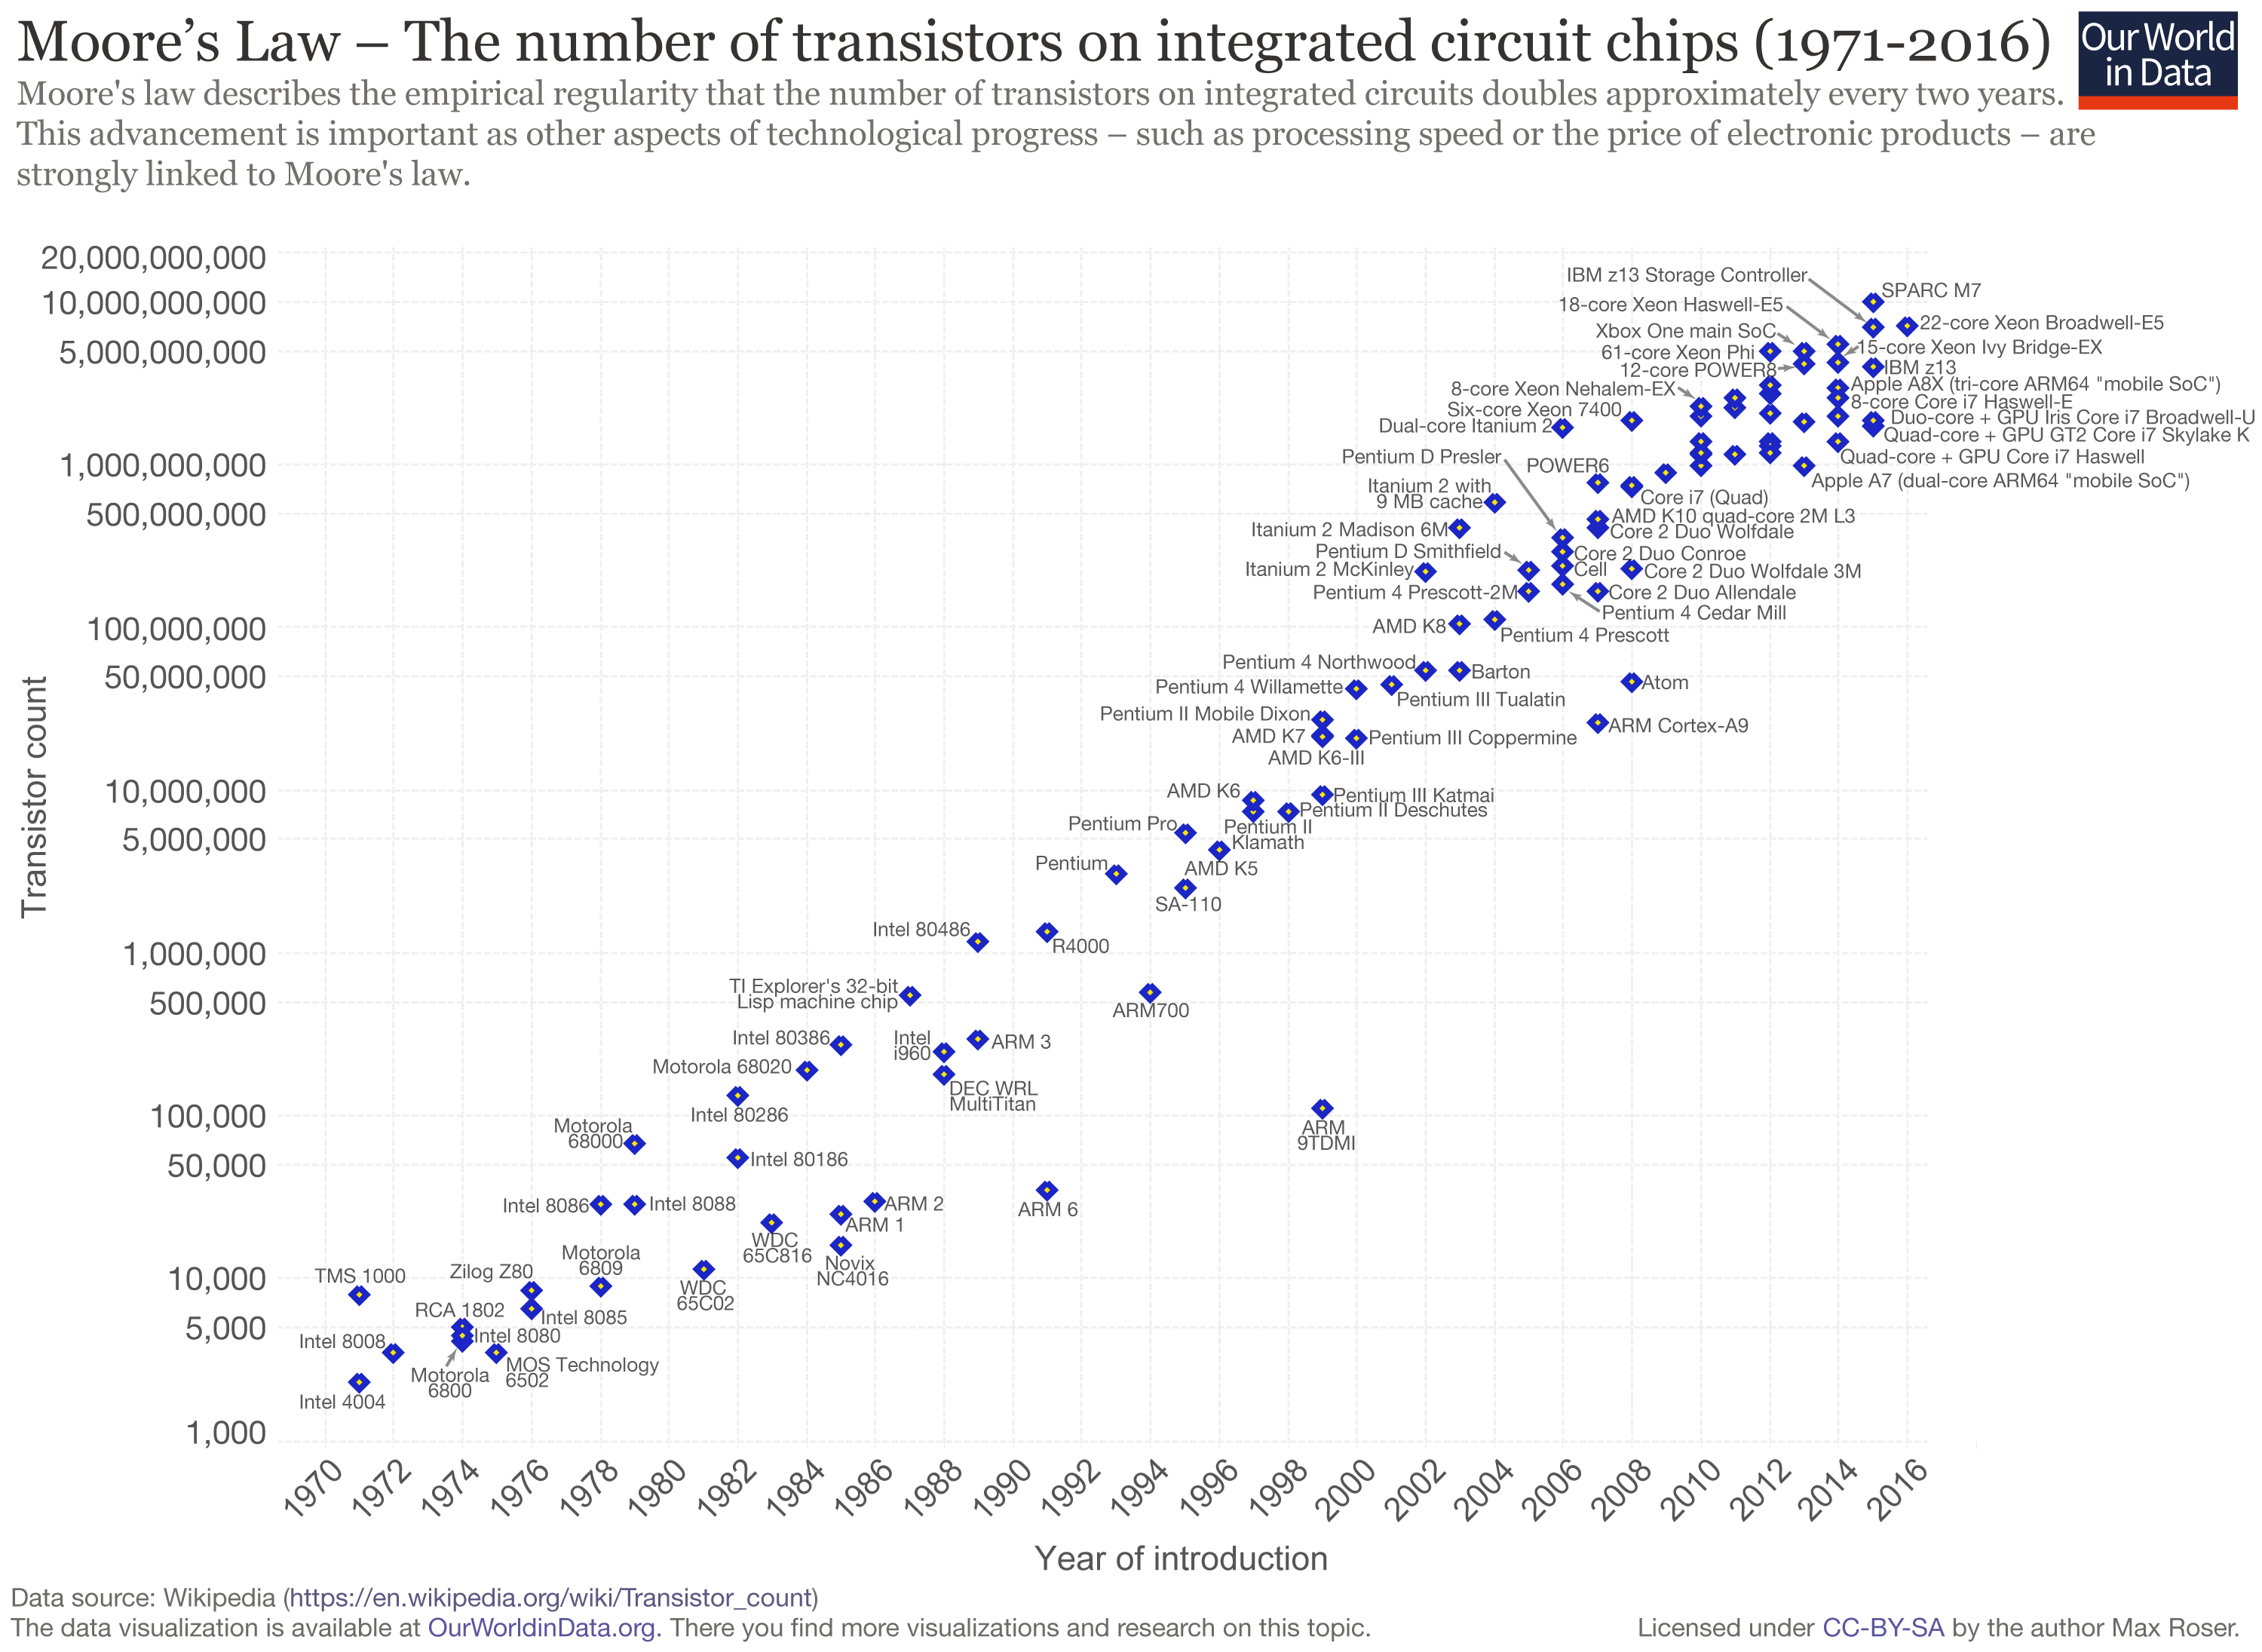
\includegraphics[width=1\linewidth]{pics/moore_law} 
\end{center} 
\caption{Plot of transistor count Vs released year for microprossesors\\ \textit{\small{Picture courtesy of  Max Roster}}}
\end{figure}

So it can been seen that transistor count has increased almost in line with Moore's prediction. But is an increase in transistor count related to an increase in complexity? The author argues that they are directly proportional; by the very definition of complexity, adding more transistors to an IC would increase its complexity. \\

Modern CPUs have upwards of 2 billions transistors \cite{2Bbeast}.

\subsection{History of operating systems, listing sizes as a proxy of complexity}
Software has also been increasing in complexity. To defend that statement a metric needs to be decided upon which can then be used to compare software from different years. Once the metric is decided, then the type of software to compare needs to be decided, as no single piece of software, to the best of the author's knowledge, has been runnable during all the years on a modern (for the relative year) CPU. \\\\

Complexity means the whole is comprised of more 'things'. A piece of software is comprised of many quantifiable things: methods, lines of code etc. Which could all have justifiable reasons for being chosen. There is also several software metrics such as cyclomatic complexity that would be ideal for this task, but for reasons of practicality it was decided on using the total space in memory the software occupies when installed. This choice was made because it was the only way to get enough data to make meaningful comparisons over the span of years.\\\\

To pick what software, or class of software to compare, it was decided the comparisons should be software that is relevant to this topic, so software designed for home computers and their modern equivalents. This rules out any firmware. Various user application have been popular throughout computers history: games, word processing, spreadsheets, communication and scientific and or engineering  programs. Games, comms and science engineering apps vary too much. Word possessors and spreadsheets could be considered but again for utilitarian reasons (it was easier to find data) another form of software for home computers was used, operating systems \ref{win_year_size_plot}. Even here the data is not completely reliable as it came from a wikipedia entry, an extremely well referenced wikipedia entry (191 references) but still unreliable.\\\\

\begin{figure} \begin{center}
\label{win_year_size_plot}
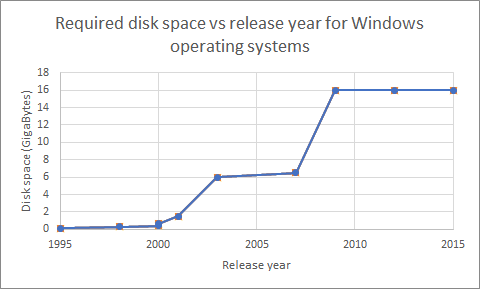
\includegraphics[width=0.8\linewidth]{pics/windows_year_size_plot} 
\end{center} 
\caption{Plot of disk space requirements to install different version of Windows operating system Vs released year\\ \textit{\small{Data provided by \cite{comp_win}}}}
\end{figure}

Others have commented on this observation before. Lawson takes a broader view, talking about the complexity of computer systems as a whole and how software effects that complexity \cite{lawson}, as well as the rise in complexity over time. Bruce Shneider has talked about the increase in complexity and its negative effects on security. Gelsinger et al. talk about the increase in software complexity driven by the need to keep up with rapid hardware changes while designinh microprossors at Intel \cite{gelsinger}. And the author suggests it would be hard to find anyone working in the industry that would disagree with the observation that software is growing increasingly complex.\\

%----------------------------------------------------------------------------------------
%----------------------------------------------------------------------------------------
\section{History of computer insecurity}
Security, defined as the freedom from hostile external forces, has been an ever increasing importance to the field of computing. The modern news is frequently running stories about data breaches, world leaders are discussing the issue and it seems like most computer users know of the concept of malware. This wasn't always the case, but sadly, it seems inevitable that every new technology will eventually be exploited by malicious people. This was indeed true for computers. \\\\

A great example, especially when talking about the history of computer security, to demonstrate the effect on society security (or lack of) can have, is the Enigma machine. Used in world war II by the Germans to great effect until Allies cracked to code in a move that has been credited with turning the war in favour of the Allies. The Enigma machine, first built in early 20C, wasn't a computer and used a electro-mechanical mechanism to encode messages, electronics where used in the Allies decoding efforts though. While not the first use of encoding and security of this sort, a more powerful example couldn't be imagined by the author. \\\\

In 1945, Rear Admiral Grace Murray Hopper fins a moth short-circuiting relays in her computer. She coins the phrases "bug" and "debugging". This is worth mentioned as its both interesting and the moth could be classified as a hostile external force, and thus has to do with security. This type of security flaw is easily solved with moth-proof covers and as such doesn't prove to be a consistent problem in the field of computers. \\\\

In 1964, malicious persons are breaking the security on AT\& T's phone network in the USA. Using 'blue boxes' and later whistles, certain tone/s can be/where produced that would allow them to make long distance calls without paying. \\\\

Now by the time the home computer era comes around, there is already a sizeable history of security. Encryption is know of and employed during this time. Firstly both users needed a private encryption key but in 1976, the first publicly available paper on public encryption keys was published \cite{diffie}. \\\\

 1979 sees the first 'worm' created, originally a research project to make computers run faster, hacker modify it to delete data from computers.  1986 brings the first virus lose in the real world, the Brain virus was never intended to be malicious and had the creators details displayed when infected.

%----------------------------------------------------------------------------------------
%----------------------------------------------------------------------------------------
\section{Malware}
Malware or malicious software can placed into a non-exhaustive, few broadly defined forms:
\begin{itemize}
\item \textbf{Worm}: a stand-alone program self-replicating program.\\
\item \textbf{Virus}: 'infects' other programs. Replicates by modifying code in other programs. Not a stand-alone program.
\item \textbf{Trojan}: program that attempts to deceive in some way. Named after the trojan horse story.
\end{itemize}

\subsection{Computer viruses}
In the 1940's John von Neumann began to developed a theory of automata, part of this theory had to do with the idea of self-replicating artificial automata \cite{neumann} or computer programs. This description sounds a lot like the malware described above; the worm or virus. Neumann himself makes repeated comparisons between computer programs and biological life \cite{neumannA}, so its no coincidence that some malware has biologically inspired names. The term 'virus' itself didn't get coined until 1987, by  Fred Cohen in his paper Computer Viruses \cite{cohen}. Cohen discusses simple viruses and points out viruses are not by nature malicious, they can be used for productive means. He uses the example of a virus program that looks for uncompressed executable files on a computer, it then asks the users permission to compresses them, prepends some code into the executable (self-replicate) and moves to the next file. As this virus program asks for the users permission, it cannot be considered malicious. But the author suggests that language is fluid and the modern meaning of a computer virus is always malicious. 

The Creeper worm is considered the first virus.

1990 self-modifying virus

\subsection{Worms}


\subsection{Trojans}


\subsection{Complexity as the root cause of modern malware susceptibility}
Fred Cohen talks about inability to protect against viruses in large systems.
Neumann talks about complexity, proves its an N-NP complete problem (I think it was him, have to read again).
